This section is split into sections describing the verification process for each module and an analysis and discussion of the overall results from the simulation.
\subsection{Verification}
\par Noise Identification Verification is done by comparing the current frame to the previous frame. The percent difference is captured and overlaid onto the output video as shown in Fig. \ref{fig:noiseIDVer}. A one unit delay block is fed as the \verb!Test! input of this block.
 \begin{figure}[H]
    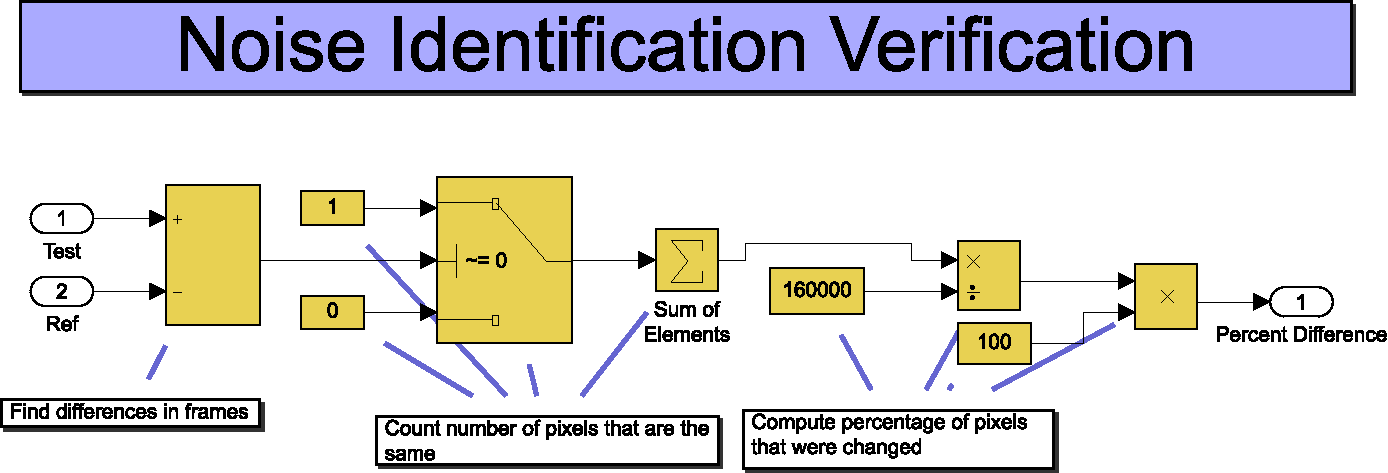
\includegraphics[width=\linewidth]{impl_dsgn_Noise Identification Verification}
    \caption{Noise Identification Verification}
    \label{fig:noiseIDVer}
\end{figure}

\par This module is verified using the peak signal-to-noise-ratio compared to the reference image. This is done in the \verb!Verification! block. The PSNR is calculated using the mean-square-error or MSE. The MSE represents the amount the reference image differs from the test image, and PSNR is a measure of the peak error and is calculated by dividing the maximum data type range by the MSE. This document uses floating point, therefore the maximum range is one\cite{mathworks}.